% !TEX root = LMThesisNicchi.tex

\chapter{Architecture and Implementation}
In this chapter we discuss the implementation of BlueTracer, providing a detailed account on how the tool is organized, on the design choices which were made during its development process, on how encountered challenges were dealt with and on the decisions which were taken to improve performance.

\section{Overview}

BlueTracer\mynote{This section requires significant extensions}, being a part of Blue Pill, is also implemented using Pin, a dynamic binary instrumentation framework by Intel, which is vastly utilized for program analysis, testing of software and in the security field. The version of Pin used for the development of the tool is 3.5, in order to benefit from the notable improvements, both in terms of execution speed and offered features, which were introduced going from the 2.14 release to the 3.x series. Pin comes with its own OS-agnostic and compiler-agnostic runtime, called PinCRT. PinCRT exposes three layers: a generic operating system interface providing basic OS services (e.g. process and thread control), together with C and C++03 (without RTTI) runtime layers, for writing instrumentation and analysis routines \cite{Pin}.   

BlueTracer has been organized primarily taking into account the rich set of APIs offered by Pin, which have led to the decision to split the tool in three parts: the first aimed at \textbf{native APIs tracing}, the second for \textbf{APIs tracing} and the last focused on \textbf{callbacks and APCs tracing} (\textit{Figure 3.1}). In particular, the tracing of native APIs also employs a different source of API information (\textit{Dr. Memory}'s system call data) than the ones utilized for tracing APIs (\textit{drltrace}'s configuration file or the information extracted from \textit{PyREbox}'s database).

This chapter will begin by describing how multi-threading was addressed in the tool, as this is central to all its components. Then, the implementation of each one of three aforementioned parts will be discussed in detail. 
\iffalse
Finally, all the configuration options of the tool will be explained.          
\fi

\begin{figure}[h]
\centering
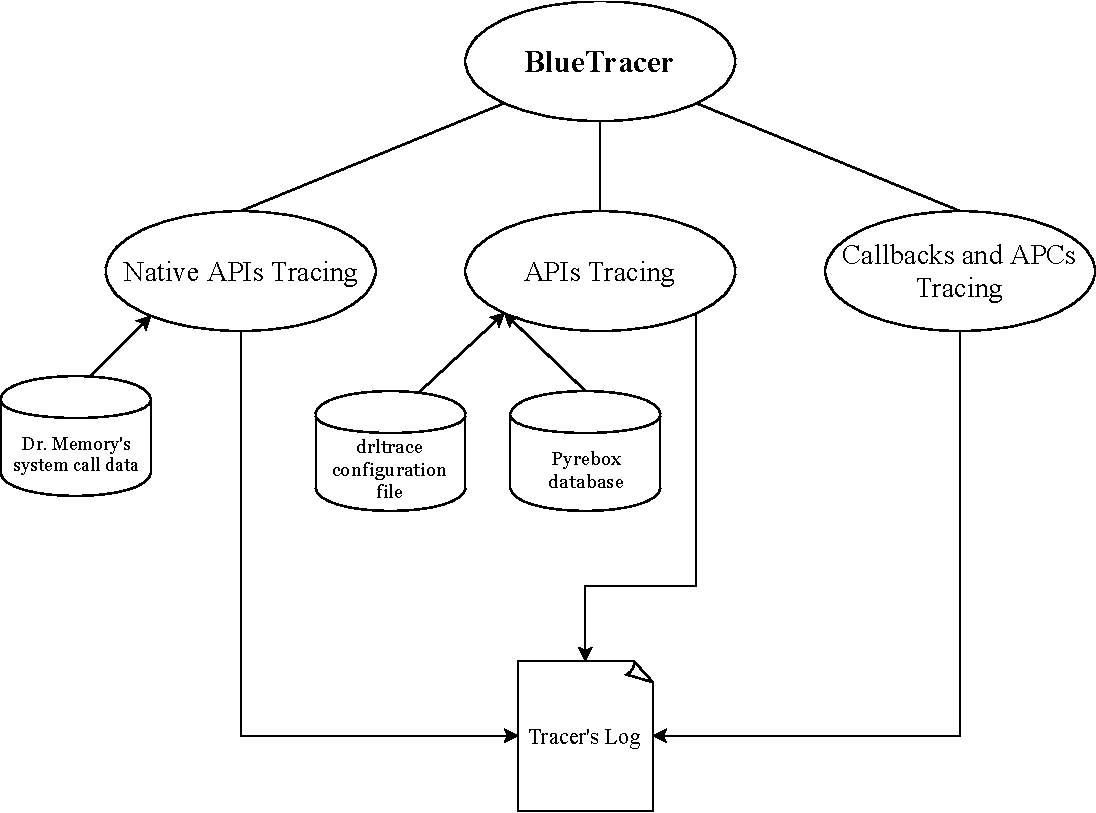
\includegraphics[width=0.85\textwidth]{Figures/BlueTracer.pdf}
\caption{\textit{BlueTracer's high level structure}}
\end{figure}

\section{Thread Management}

Since the samples under analysis are typically multithreaded applications, let us go through the mechanisms exposed by Pin to manage threads and how those were employed in the implementation of the tool.

Pin assigns to each thread an ID, a small number beginning at 0
which is not the same as the operating system thread ID. A way to obtain such ID is by using as analysis routine argument \texttt{IARG\_THREAD\_ID}, which passes the thread ID assigned by Pin for the calling thread. This ID is typically used as an index of an array of thread data.
In fact, the Pin API makes available an efficient thread local storage (TLS). In order to utilize it, it is first required to allocate a new TLS key via \texttt{PIN\_CreateThreadDataKey}, which can optionally take as input a pointer to a destructor function. After that, any thread of the process can use the TLS key, in addition to its Pin-specific thread ID, to store (\texttt{PIN\_SetThreadData}) and retrieve (\texttt{PIN\_GetThreadData}) values in its own slot. The starting value relative to the key in every thread is \texttt{NULL}.
Pin makes also available call-backs when each thread starts (registered with \texttt{PIN\_AddThreadStartFunction}) and ends (registered with \texttt{PIN\_AddThreadFiniFunction}). This is typically where thread local data is allocated, manipulated and stored in a thread's local storage\cite{Pin}.

In BlueTracer, each TLS slot stores a \texttt{struct} of the type \texttt{bluepill\_tls} (\textit{Listing 3.1}) for every thread. Such \texttt{struct} is dynamically allocated every time a thread starts in the \texttt{OnThreadStart} callback function and is consequently deallocated in the \texttt{onThreadFini} function when the thread ends.

\vspace{0.5cm}
\begin{lstlisting}[caption={Thread Local Data},captionpos=b]
typedef struct {
 ...
 syscall_tracer* syscallEntry;     // Pointer to NTAPI entry
 vector<stackEntry>* shadowStack;  // Shadow stack
 uint call_number;             	   // Calls counter							
 
 buf_info_t* buffer;		   	   // Buffer for writing to file				 
 FILE* OutFile;                    // Output file pointer
 
 // Pointer to function for opening file/writing to file	
 void(*file_write)(THREADID, buf_info_t*, FILE*, const char*, 	...);
 
 ...
} bluepill_tls;
\end{lstlisting}

Since the first three fields of the above \texttt{struct} (lines 3-5) are employed when tracing native APIs and APIs, they will be discussed in detail later in the chapter. Now let us focus on the remaining fields, which are used by BlueTracer to write the traced information in the appropriate log files. 

\subsection{Log Files and Multithreading}

In BlueTracer, the traced data is written to a binary file, one for every thread. The default naming convention used for the tracer's log files is \texttt{Traced.[OS Process ID].[Pin-specific Thread ID]}, similarly to the one Blue Pill employs in its own log files, with the user being able to change \texttt{Traced} with a name of its choice in the configuration file. 

When writing data to file, each thread invokes the \texttt{file\_write} function, whose pointer is located in the instance of the \texttt{bluepill\_tls} struct associated to the thread (line 11 of \textit{Listing 3.1}). However, such data, which follows the same format of strings used by \texttt{fprintf}, is not directly written to file. Instead, an intermediate 8 kB buffer is used (line 7 of \textit{Listing 3.1}): only when the buffer is full (or when the amount of data to be written does not fit the buffer) file writing actually occurs. The choice of using a buffer was made as an attempt to improve performance, as it allows the aggregation of small write operations into a block size that is more efficient for the disk subsystem.

A problem which was encountered when trying to conjugate file management and multithreading is that there exists a known isolation issue affecting Pin on Windows. Specifically, it is possible for a deadlock to take place if a file is opened in a callback in the context of multithreaded applications. As a result of this issue, it is not possible to open the tracer's log file in the \texttt{OnThreadStart} callback. Pin's manual proposes to circumvent the problem by opening the file in the \texttt{main} and tagging the data with the thread ID \cite{Pin}. However, this conflicts with the idea of having one file for each thread.

In order to bypass this limitation of the Pin's framework, the following strategy was employed:
\begin{enumerate}
\item When initializing the thread local data in \texttt{OnThreadStart}, \texttt{file\_write} is set to point to a function named \texttt{file\_open}.
\item The first time a thread attempts to write data to file \texttt{file\_open} is invoked.
\item \texttt{file\_open} carries out the following actions:
\begin{enumerate}
\item Opens the tracer's log file (this is safe since the file is not opened in a callback)
\item Sets the obtained file pointer in the thread local data (line 8 of \textit{Listing 3.1})
\item Adds the data to be written in the buffer (which is eventually written to file if the buffer is too small to hold it)
\item Sets \texttt{file\_write} to point to \texttt{buf\_write}, a function which is in charge of just writing data to the buffer and to file.
\end{enumerate}
\item As a result of this, when the thread attempts to write to file again, \texttt{buf\_write} is invoked, thus allowing the thread to just write to file without going through opening the file again.   
\end{enumerate}   

\section{Native APIs Tracing}
\iffalse
Talk about log structure when talking about how arguments are printed
\fi

Windows Native APIs are employed to call operating system services in kernel mode in a controlled way.  
In fact, all core Windows components, which possess direct access to hardware and services in charge of handling the computer's resources (e.g. memory), operate in kernel mode. This means that, every time a user mode application desires to carry out certain actions, like for instance starting a thread or allocating virtual memory, they must rely on kernel mode  services. The Windows Native API corresponds to the system call interface of standard monolithic operating systems, such as the majority of UNIX-like systems, with the difference that in the latter case the system call interface is documented and can be utilized directly by applications. Instead, due to Windows' architecture, Windows Native APIs are concealed to the programmer by the higher level Windows (\texttt{Win32}) APIs \cite{NTAPI1}. User mode Windows Native APIs, which are identified by their \texttt{Nt} prefix and are exported by \texttt{ntdll}, have caught the attention of malware writers since they are seen as a way of bypassing the documented APIs with the objective of performing a series of actions without being discovered \cite{NTAPI2}. For this reason it is a good idea to also trace them, in addition to the ordinary Windows APIs.  

Pin provides a set of APIs aimed at assisting the extraction of information relative to the system calls made by the pinned application, also including information relative to Windows Native APIs. In particular, in Blue Pill (and consequently in BlueTracer) \texttt{PIN\_AddSyscallEntryFunction} and  \texttt{PIN\_AddSyscallExitFunction} were used for this purpose. In fact, these allow to register notification functions which are called immediately before and after the execution of a system call \cite{Pin}. In BlueTracer, the function in charge of gathering Native API information before execution is \texttt{TraceSysCallEntry} while the one responsible for collecting Native API information after execution is \texttt{TraceSysCallExit}. They have been both been embedded in Blue Pill's notification functions and their overall structure is detailed in \textit{Figure 3.2}.
\\
\begin{figure}[h]
\centering
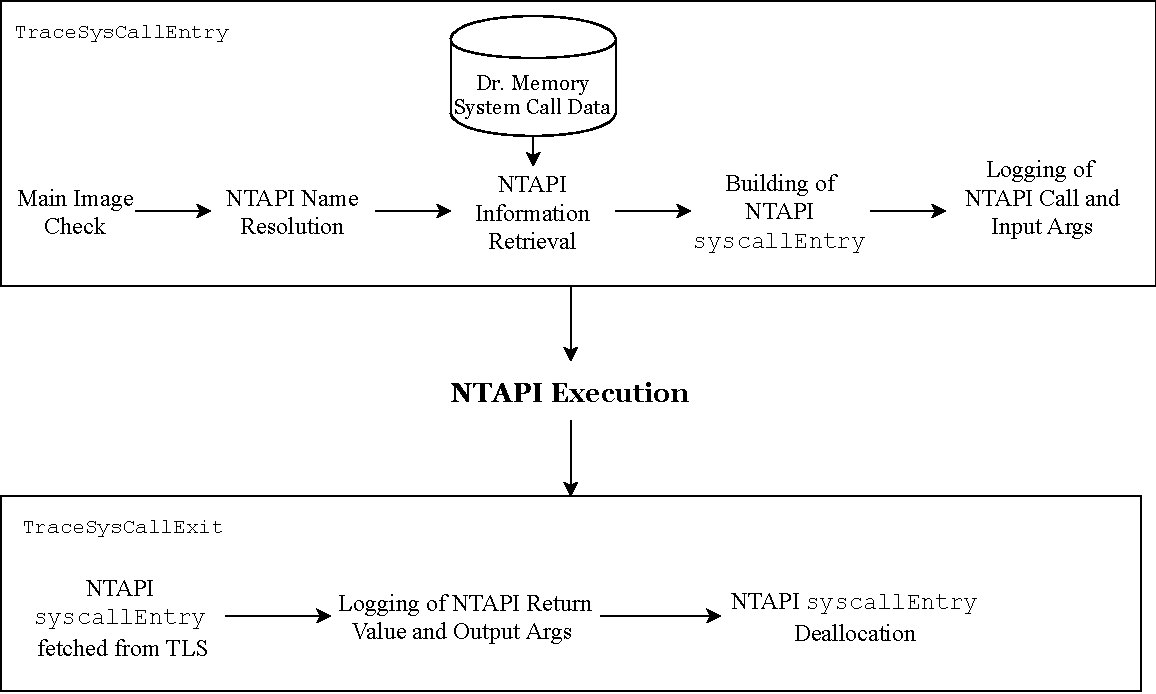
\includegraphics[scale=0.75]{Figures/NTAPITracing.pdf}
\caption{\textit{Native APIs Tracing Workflow}}
\end{figure}
\\
Following \textit{Figure 3.2}, let us now thoroughly analyze the main steps which take place when Native APIs are traced.

\subsection{Main Image Check}
In order to filter the logged information relative to Native APIs, BlueTracer allows the analyst to decide, through the use of a boolean parameter (\texttt{MainImage}) in the configuration file, whether or not only Native APIs called invoked directly from the main executable of the pinned application should be traced. Therefore, as it can be seen in \textit{Figure 3.2}, the first thing which is done in \texttt{TraceSysCallEntry}, assuming that the \texttt{MainImage} configuration parameter has been set to \texttt{true}, is to determine if the Native API call is taking place directly from the main executable.

To this end, Pin's \texttt{IMG} APIs are employed, where in Pin an \texttt{IMG} represents all the data structures relative to binaries and shared libraries \cite{Pin}. Specifically, in Blue Pill, \texttt{IMG\_AddInstrumentFunction} is utilized to register a callback which is invoked each time an image is loaded. Inside such callback, which takes as one of the input parameters the \texttt{IMG} object representing the image being loaded, the following steps are taken:
\begin{enumerate}
\item \texttt{IMG\_IsMainExecutable} is employed to determine if the image being loaded is the main executable of the pinned application.
\item If this is the case, \texttt{IMG\_HighAddress} and \texttt{IMG\_LowAddress} are invoked. These two APIs return the highest address and the lowest address respectively of any code or data loaded by the image corresponding the the \texttt{IMG} object they take as input. By employing these APIs is therefore possible to determine the address range relative to the main executable. 
\end{enumerate}  

Having obtained the main executable address range in this way, it is then employed in \texttt{TraceSysCallEntry} to learn if the Native API call is occuring directly from the main image. Internally, before entering kernel mode every Native API executes some common code, i.e. each Native API stores its ordinal in the \texttt{eax} register and invokes \texttt{KiFastSystemCall}, where the \texttt{sysenter} instruction is used to actually enter kernel mode. When \texttt{sysenter} is executed, the kernel obtains the ordinal number from \texttt{eax} and utilizes it to call the corresponding function, prior to going back to user mode \cite{MalwareTech}.

In Pin, the Native API is intercepted right before \texttt{sysenter} is executed. This could be inferred by the fact that, in \texttt{TraceSysCallEntry}, the instruction pointer (obtainable via the \texttt{PIN\_GetContextReg} API) contains \texttt{sysenter}'s address. In light of this, in addition to the fact that each Native API calls \texttt{KiFastSystemCall} without setting a stack frame, the application's stack during the execution of \texttt{TraceSysCallEntry} is in the following state (\textit{Figure 3.3}).
\\
\begin{figure}[h]
\centering
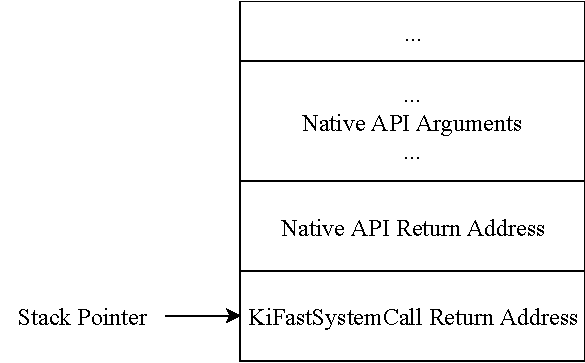
\includegraphics[width=0.7\textwidth]{Figures/StackMainImage.pdf}
\caption{\textit{Stack before} \texttt{sysenter} \textit{execution}}
\end{figure}     

Having outlined the general situation, it is finally possible to describe how the main image check is carried out:

\begin{enumerate}
\item The first check involves discovering whether or not \texttt{sysenter} is called directly from the main executable. As Pin intercepts Native APIs right before the execution of \texttt{sysenter}, this can be trivially done by checking if the instruction pointer value obtained in \texttt{TraceSysCallEntry} falls within the main executable memory address range.
\item Secondly, it is required to examine if the Native API return address belongs to the main executable. As a result of what shown in \textit{Figure 3.3} such return address is obtained by adding 4 to the stack pointer and retrieving the pointed value, where the stack pointer can be obtained in Pin through the use of \texttt{PIN\_GetContextReg}. The resulting value is then, once more, compared with the main executable memory address range.
\end{enumerate}

\subsection{Native API Name Resolution}

Previously, it was stated how it is possible to register a callback function to be executed before Native APIs through the use of \texttt{PIN\_AddSyscallEntryFunction}. Such callback functions, named \texttt{SYSCALL\_ENTRY\_CALLBACK}s, receive a set of parameters, including \texttt{ctx}, the application's register state immediately before the system call execution, and \texttt{std}, the system call standard. In Blue Pill, these two parameters are used to invoke \texttt{PIN\_GetSyscallNumber} inside its \texttt{SYSCALL\_ENTRY\_CALLBACK}. Such API returns the number (ID) of the Native API to be executed in the provided context \cite{Pin}.

Blue Pill employs a mechanism which allows it to obtain the Native API name from its number, since the hooking functions it employs are indexed by name and not by ordinal. This choice was made because the identifiers vary depending on the Windows version, even among different Service Pack versions. For the same reason, the information needed by BlueTracer to correctly log Native APIs is also indexed by Native API name and, consequently, BlueTracer also utilizes the aforementioned Native API name resolution mechanism.

The idea is to create an array, named \texttt{syscallIDs}, where Native API names are indexed by their IDs, by parsing \texttt{ntdll}'s export information. The export data of a PE is stored in the \texttt{IMAGE\_EXPORT\_DIRECTORY} structure located in the header. In our case, the most relevant fields of this structure are:

\begin{itemize}
\item The \texttt{AddressOfFunctions} array, which contains RVAs \footnote{A RVA (Relative Virtual Address) is essentially an offset within the PE image in memory} pointing to the actual exported functions and is indexed by an export ordinal.
\item The \texttt{AddressOfNames} array, which is an array of 32-bit RVAs pointing to symbol strings.
\item The \texttt{AddressOfNameOrdinals} array, which is an array of 16-bit ordinals existing in parallel with \texttt{AddressOfNames}, i.e. they possess the same number of elements and there is a direct relation between equivalent indices \cite{Sikorski:2012:PMA:2181153}.  
\end{itemize}

\newpage

With this in mind, \texttt{syscallIDs} is built by carrying out the following actions for every element \texttt{iName} in \texttt{AddressOfNames}:

\begin{enumerate}
\item The corresponding \texttt{AddressOfNameOrdinals} element is retrieved, i.e. the one with the same index. Let us call this value \texttt{iOrdinal}.
\item \texttt{iOrdinal} is used to index in \texttt{AddressOfFunctions}. This time the obtained value is the RVA pointing to the exported function.
\item The pointed function is expected to begin \texttt{mov eax, syscall\_number}. As a result of this, the first byte should be \texttt{B8h} and the syscall number can be obtained by considering the next four bytes.  
\end{enumerate}

By following the above procedure, every element in \texttt{AddressOfNames} can be therefore mapped to the corresponding identifier. 

\subsection{Native API Information Representation and Retrieval}

When tracing Native APIs, it is wanted to record as much data as possible as well as correctly formatting the arguments' values. To do this, it is required to have access to some kind of source of Native API related information, which can assist the tracer in the logging activity by, for example, providing the number of arguments a Native API takes as input, listing the arguments' types and differentiating between input and output arguments.
In BlueTracer, this information was adapted from the Native API data provided by Dr.Memory \cite{DrMemory}, a memory monitoring tool based on the DynamoRIO DBI framework.

For each Native API, the information related to it is contained in a \texttt{struct} of type \texttt{syscall\_info\_t} (\textit{Listing 3.2}). Most fields of such \texttt{struct} are self-explanatory. In particular, \texttt{num} is a \texttt{struct} storing two values indicating the system call number; these are filled in dynamically by Dr.Memory but are not needed by BlueTracer. Furthermore, the \texttt{flags} field is utilized to notify whether or not all the details of the Native API are known, as most Native APIs are undocumented. Undoubtedly though, a major role is played by the \texttt{arg} array, which is made up by \texttt{sysinfo\_arg\_t} \texttt{struct}s (\textit{Listing 3.2}) containing the data of the Native API arguments. This array is initialized with size \texttt{MAX\_ARGS\_IN\_ENTRY} (i.e. 18), since a Native API can have at most 18 arguments. 
\\
\begin{lstlisting}[caption={\texttt{struct} containing Native API-related information},captionpos=b]
	typedef struct _syscall_info_t {

		drsys_sysnum_t num;			// Native API ID
		const char *name;			// Native API Name
		uint flags; 				// SYSINFO_ flags
		uint return_type; 			// Return type
		int arg_count;				// Number of arguments

		// Array of arguments
		sysinfo_arg_t arg[MAX_ARGS_IN_ENTRY];

		...
	} syscall_info_t;
\end{lstlisting}

\begin{lstlisting}[caption={\texttt{struct} containing information associated to a Native API argument},captionpos=b]
	typedef struct _sysinfo_arg_t {
		int param; 				    // Parameter Ordinal
		int size; 				    // Size
		uint flags; 				// SYSARG_ flags
		int type; 				    // Type
		const char *type_name; 	    // Symbolic Name of the arg Type
	} sysinfo_arg_t;
\end{lstlisting}

In \texttt{sysinfo\_arg\_t}, other than \texttt{param} and \texttt{size}, that are straightforward, the following fields are also present:
\begin{itemize}
\item \texttt{flags}, which stores an \texttt{OR} of flags describing the argument's characteristics. The most important ones are:

\begin{itemize}
\item \texttt{SYSARG\_READ (R)} : input argument. 
\item \texttt{SYSARG\_WRITE (W)} : output argument.
\item \texttt{SYSARG\_INLINED} : non-memory argument, i.e the whole value is in parameter slot.
\item \texttt{SYSARG\_HAS\_TYPE (HT)} : argument with a type specifier. In fact, a non \texttt{SYSARG\_INLINED} argument is by default of type \texttt{struct} (\texttt{DRSYS\_TYPE\_STRUCT}), unless specified otherwise by \texttt{SYSARG\_HAS\_TYPE}. 
\end{itemize}

\item \texttt{type}, which is an \texttt{enum} value indicating the data type of the parameter

\item \texttt{type\_name}, a string indicating the symbolic name of the \texttt{arg} type, which is typically filled dynamically based on the \texttt{type} value. In case the argument value is a named constant, the \texttt{type\_name} field contains the name of the enumeration the constant belongs to. In fact, for each one of these enumerations, BlueTracer has access to a \texttt{struct} specific for that enumeration containing the constant values and their corresponding name. This information was also provided by Dr.Memory and is employed to translate constants to the appropriate name, as it will be explained in the next section. 

\end{itemize}

To make things clearer, an instance of \texttt{syscall\_info\_t} for the Native API \texttt{NtAllocateVirtualMemory} was provided in the listing below (\textit{Listing 3.4}).
\\
\begin{lstlisting}[caption={Instance of \texttt{syscall\_info\_t} relative to \texttt{NtAllocateVirtualMemory}},captionpos=b]
	{ { 0,0 },"NtAllocateVirtualMemory", OK, RNTST, 6,
	{
		{ 0, WIN_SIZE(HANDLE), SYSARG_INLINED, DRSYS_TYPE_HANDLE },
		{ 1, WIN_SIZE(PVOID), R | WR | HT, DRSYS_TYPE_POINTER },
		{ 2, WIN_SIZE(ULONG), SYSARG_INLINED, DRSYS_TYPE_UNSIGNED_INT },
		{ 3, WIN_SIZE(ULONG), R | WR | HT, DRSYS_TYPE_UNSIGNED_INT },
		{ 4, WIN_SIZE(ULONG), SYSARG_INLINED, DRSYS_TYPE_UNSIGNED_INT, "MEM_COMMIT" },
		{ 5, WIN_SIZE(ULONG), SYSARG_INLINED, DRSYS_TYPE_UNSIGNED_INT, "PAGE_NOACCESS" },
	}
\end{lstlisting}

In \textit{3.2.2} it was explained how BlueTracer obtains a Native API name from its ID. After that, as shown in \textit{Figure 3.2}, there must be a way to, given a specific Native API name, retrieve the corresponding \texttt{syscall\_info\_t struct}. This is done by building an hash map during the tool's initialization which maps the Native API name to the appropriate \texttt{struct}. Such idea is also adopted for named constants enumerations since a hash map is also constructed with the objective of associating the name of a named constant enumeration to the corresponding \texttt{struct}.    

\subsection{Native API Logging}
With reference to \textit{Figure 3.2}, let us consider the point in \texttt{TraceSysCallEntry} where the \texttt{syscall\_info\_t struct} relative to the Native API being traced was successfully retrieved. Before describing how the logging of "known" Native APIs is performed, it is worth mentioning that, in case a \texttt{struct} describing a certain Native API is not found, BlueTracer just logs the name of the Native API and the input value of a user-specified number of arguments (4 by default).

The first step towards logging "known" Native APIs is allocating and initializing a \texttt{syscall\_tracer struct} (\textit{Listing 3.5}) representing the specific Native API being traced. This \texttt{struct} is built starting from the data present in the previously retrieved  \texttt{syscall\_info\_t struct} and it is at the heart of the logging of the Native API.
\\
\begin{lstlisting}[caption={\texttt{struct} representing the Native API being traced},captionpos=b]
	typedef struct _syscall_tracer {
		ADDRINT syscall_number;			// Native API ID
		const char * syscall_name;		// Native API Name
		int argcount;				    // Number of Arguments

		// Array of arguments
		drsys_arg_t arguments[MAX_ARGS_IN_ENTRY];

		drsys_arg_t retval;			    // Return value
		int syscall_counter;			// Native API Counter
	} syscall_tracer;
\end{lstlisting}

Even for \texttt{syscall\_tracer}, each field is self-explanatory. The only one which was not encountered before is the \texttt{syscall\_counter} field. The rationale behind this field is that, in the log, each traced call has a unique integer associated to it, utilized to group together the information relative to the call in post-processing. The next identifier to be assigned is stored in the \texttt{call\_number} field of the thread local storage (\textit{Listing 3.1}). Therefore, \texttt{syscall\_counter} simply contains the unique identifier associated to the Native API in the log. The arguments of a specific Native API are represented via the \texttt{drsys\_arg\_t} struct (\textit{Listing 3.6}).
\\
\begin{lstlisting}[caption={\texttt{struct} representing the an argument of the Native API being traced},captionpos=b]
typedef struct _drsys_arg_t {

	// Whether operating pre-call (if true) or post-system call (if false)
	bool pre;

	int ordinal;			    // Parameter Ordinal				
	int size;			        // Size	
	uint flags;			        // SYSARG_ flags
	int type;			        // Type
	const char *type_name;		// Symbolic Name of the arg Type

	// String describing the symbolic name of a named constant's enum
	const char *enum_name;

	// Argument value
	ADDRINT value;
	
} drsys_arg_t
\end{lstlisting}

\texttt{drsys\_arg\_t}'s fields are mostly the same of \texttt{sysinfo\_arg\_t}, with three additions:
\begin{itemize}
\item \texttt{pre}, which is a boolean flag set to \texttt{true} when the logging is occurring before the Native API is executed (i.e. in \texttt{TraceSysCallEntry} and set to false when the logging is occurring after the Native API is executed (i.e. in \texttt{TraceSysCallExit}).
\item \texttt{enum\_name}, a string containing the symbolic name of the enumeration a named constant belongs to. In most cases, this is the symbolic name associated to the first constant of the enumeration. Such field was introduced to decouple type name and enumeration name.
\item \texttt{value}, an \texttt{ADDRINT}\footnote{The ADDRINT type is defined by Pin and represents a memory address} containing the value of the argument. This is obtained through the \texttt{PIN\_GetSyscallArgument} API, which takes as input the context before the execution of the system call, the system call standard and the ordinal number of the argument whose value is requested.  
\end{itemize}

As previously mentioned in section 3.1.1, each thread possesses its own log file, whose pointer resides in the thread local storage, and writes on it by means of the \texttt{file\_write} function, also located in the thread local storage (\textit{Listing 3.1}). The first Native API component being logged is its name and this is done with the following format:
\\ 
\texttt{\textasciitilde\textasciitilde[System ID of thread]\textasciitilde\textasciitilde} \texttt{ [Call Counter] [Image Name]![Native API Name]}  
In the context of Native APIs, the name of the image is always \texttt{ntdll}, but this is not the case when tracing APIs.

Argument logging is done via the \texttt{print\_arg} function (\textit{Listing 3.7}), which is structured as follows:

\begin{itemize}
\item Firstly, it is determined if the argument being logged is a named constant, i.e. it is checked if \texttt{enum\_name} is different from \texttt{NULL}. In that case, the \texttt{get\_arg\_syname} function is invoked, which is in charge of, given the input named constant value, finding the corresponding name and recording it to the log. The named constant resolution is carried out by initially fetching the \texttt{struct} containing all the members of the enumeration the named constant belongs to, through the use of the aforementioned hash map. Then, it is determined if there is a perfect match between the argument value and one of the values of the \texttt{struct}'s entries. If this occurs, then the associated symbolic name is simply retrieved from the \texttt{struct}'s entry. Otherwise, a linear search is performed to unveil possible composite named constants (e.g. \texttt{FILE\_SHARED\_READ | FILE\_SHARED\_WRITE}).    

\end{itemize}

\vspace{1em}
\begin{lstlisting}[caption={\texttt{print\_arg} function},captionpos=b]
static void print_arg(drsys_arg_t* curr_arg, bluepill_tls* tdata, uint syscall_counter) {

	...

	// Constant Resolution
	if (curr_arg->enum_name != NULL) {
		if (get_arg_symname(curr_arg, tdata))
			return;
	}

	switch (curr_arg->type) {
		case DRSYS_TYPE_VOID:	      print_simple_value(curr_arg, true, tdata); break;
		case DRSYS_TYPE_POINTER:      print_simple_value(curr_arg, true, tdata); break;
		case DRSYS_TYPE_BOOL:         print_simple_value(curr_arg, false, tdata); break;
		case DRSYS_TYPE_INT:          print_simple_value(curr_arg, false, tdata); break;
		case DRSYS_TYPE_SIGNED_INT:   print_simple_value(curr_arg, false, tdata); break;
		case DRSYS_TYPE_UNSIGNED_INT: print_simple_value(curr_arg, false, tdata); break;
		case DRSYS_TYPE_HANDLE:       print_simple_value(curr_arg, false, tdata); break;
		case DRSYS_TYPE_NTSTATUS:     print_simple_value(curr_arg, false, tdata); break;
		case DRSYS_TYPE_ATOM:         print_simple_value(curr_arg, false, tdata); break;
	default: {
		if (curr_arg->value == 0) {
			(tdata->file_write)(tdata->threadid, tdata->buffer, tdata->OutFile, "<null>");
		}
		else if (curr_arg->pre && !TEST(SYSARG_READ, curr_arg->flags)) {
			(tdata->file_write)(tdata->threadid, tdata->buffer,
			tdata->OutFile, PFX, curr_arg->value);
		}
		else {
			if (!print_known_compound_type(curr_arg, tdata))
				(tdata->file_write)(tdata->threadid, tdata->buffer, tdata->OutFile, "<NYI>");
		}
	}
	...
}
\end{lstlisting}

\begin{itemize}
\item Then, if the argument's type is primitive (e.g. \texttt{int}, \texttt{bool}, etc.),  \texttt{print\_simple\_value} is invoked to record its value. In particular the second parameter of this function is a boolean which is set to \texttt{true} if it is wanted to print the argument's value with leading zeros (e.g. if the argument is of pointer type and the address it stores is being logged ) and \texttt{false} otherwise. The way \texttt{print\_simple\_value} operates is quite straightforward:
\begin{enumerate}
\item At the beginning the argument's value is simply logged, with leading zeroes or not depending on the previously mentioned parameter
\item Then, if the argument is a pointer, it is determined if the value it points to needs to be logged. This occurs if the argument is being processed before the Native API execution (i.e. \texttt{pre} is \texttt{true}) and is an input parameter (i.e. SYSARG\_READ is contained in \texttt{flags}) or if the argument is being processed after the Native API execution (i.e. \texttt{pre} is \texttt{false}) and is an output parameter (i.e. SYSARG\_WRITE is contained in \texttt{flags}). The pointed value is obtained through the use of \texttt{PIN\_SafeCopy}, which copies the specified number of bytes from a source memory region to a destination memory region, guaranteeing safe return to the caller even if such regions are inaccessible.  
\end{enumerate}      

\item Finally, if the argument's type is not a primitive one, it is checked if it is \texttt{null} and if it is a complex output parameter being traced before the Native API execution, situation in which only the address stored in the pointer is logged. If none of these two scenarios are true, then the tracer finds itself in the situation where it is required to log the value of a complex type. This is performed through the invocation of \texttt{print\_known\_compound}. As of right now, such function differentiates between four complex types, namely \texttt{UNICODE\_STRING}, \texttt{OBJECT\_ATTRIBUTES}, \texttt{IO\_STATUS\_BLOCK} and \texttt{LARGE\_INTEGER}, and logs the argument's value accordingly. If the argument's type is a complex type that is not supported, the symbolic value \texttt{<NYI>} (not yet implemented) is recorded.    

\end{itemize}

Once the arguments' input values are logged, then the reference to the \texttt{syscall\_tracer struct} representing the Native API under analysis is stored in thread local data (\textit{Listing 3.1}). This is done so that, after the Native API's execution, the corresponding \texttt{syscall\_tracer} data structure can be accessed from \texttt{TraceSysCallExit}. In fact, as mentioned in section 3.2, the \texttt{bluepill\_tls struct} associated to the running thread can be retrieved in any analysis function by means of \texttt{PIN\_GetThreadData}.

In \texttt{TraceSysCallExit}, after the value of \texttt{syscallEntry} has been fetched from the thread local storage, then it is determined whether the Native API has succeeded by checking if the output of \texttt{PIN\_GetSyscallErrno} is equal to zero, where \texttt{PIN\_GetSyscallErrno} is a Pin API returning the error code of the system call which has just returned with the provided context. Afterwards, \texttt{PIN\_GetSyscallReturn} is utilized to get the return value of the Native API and, with this information, the corresponding \texttt{drsys\_arg\_t} data structure is built. Successively, the Native API return value is logged, together with the output arguments, using once again \texttt{print\_arg} (\textit{Listing 3.7}). Finally, the \texttt{syscall\_tracer struct} representing the Native API being traced is deallocated.

To conclude this section, let us show how a traced Native API looks like in the log file (\textit{Figure 3.4}). As it can be observed, the adopted log format is quite intuitive. In fact, the idea was to have a log which is both easy to read by the analyst but also easy to parse and post-process.      
\\

\lstset{
    language=C++,
    frame=tb, % draw a frame at the top and bottom of the code block
    tabsize=4, % tab space width
    showstringspaces=false, % don't mark spaces in strings
    numbers=none, % display line numbers on the left
    commentstyle=\color{ao}, % comment color
    keywordstyle=\color{blue}, % keyword color
    stringstyle=\color{red}, % string color
    basicstyle=\footnotesize\ttfamily,
    basewidth = {.48em}
}
\begin{lstlisting}[caption={Log relative to a \texttt{NtOpenFile} call},captionpos=b]
~~2868~~ 1072 ntdll.dll!NtOpenFile
1072 	arg 0: 0x000fe810 (type=HANDLE*, size=0x4)
1072 	arg 1: 0x100020 (type=unsigned int, size=0x4)
1072 	arg 2: len=0x18, root=0x0, name=210/538 "\??\C:\Windows\WinSxS\
		x86_microsoft.windows.gdiplus_6595b64144ccf1df_1.1.7601.23894_none_5c0be957a009922e", 
		att=0x40, sd=0x00000000, sqos=0x00000000 (type=OBJECT_ATTRIBUTES*, size=0x4)
1072 	arg 3: 0x000fe7c0 (type=IO_STATUS_BLOCK*, size=0x4)
1072 	arg 4: FILE_SHARE_READ|FILE_SHARE_WRITE (type=named constant, value=0x3, size=0x4)
1072 	arg 5: FILE_DIRECTORY_FILE|FILE_SYNCHRONOUS_IO_NONALERT
 		(type=named constant, value=0x21, size=0x4)
1072    succeeded =>
1072 	arg 0: 0x000fe810 => 0x58 (type=HANDLE*, size=0x4)
1072 	arg 3: status=0x0, info=0x1 (type=IO_STATUS_BLOCK*, size=0x4)
\end{lstlisting}
\lstset{
    language=C++,
    frame=tb, % draw a frame at the top and bottom of the code block
    tabsize=4, % tab space width
    showstringspaces=false, % don't mark spaces in strings
    numbers=left, % display line numbers on the left
    commentstyle=\color{ao}, % comment color
    keywordstyle=\color{blue}, % keyword color
    stringstyle=\color{red}, % string color
    basicstyle=\footnotesize\ttfamily,
    basewidth = {.48em}
}

\section{APIs Tracing}

In Microsoft Windows, APIs are implemented as functions provided by a set of dynamic-link libraries. These, also known as DLLs, constitute Microsoft's way of implementing the concept of shared libraries in the Windows operating system. Therefore, the functions they make available can be employed by different applications \cite{DLL}. Windows APIs offer a plethora of functionalities which belong to many different categories, ranging from base services (e.g. file management) to user interface functions and network operations \cite{WinAPI}. In light of this, a Windows API has rich semantic information associated to it and tracing the sequence of APIs a malware calls provides analysts with a very high-level view of the sample's behavior. This is why BlueTracer's API tracer component is undoubtedly the most important one. 
\\
\begin{figure}[h]
\centering
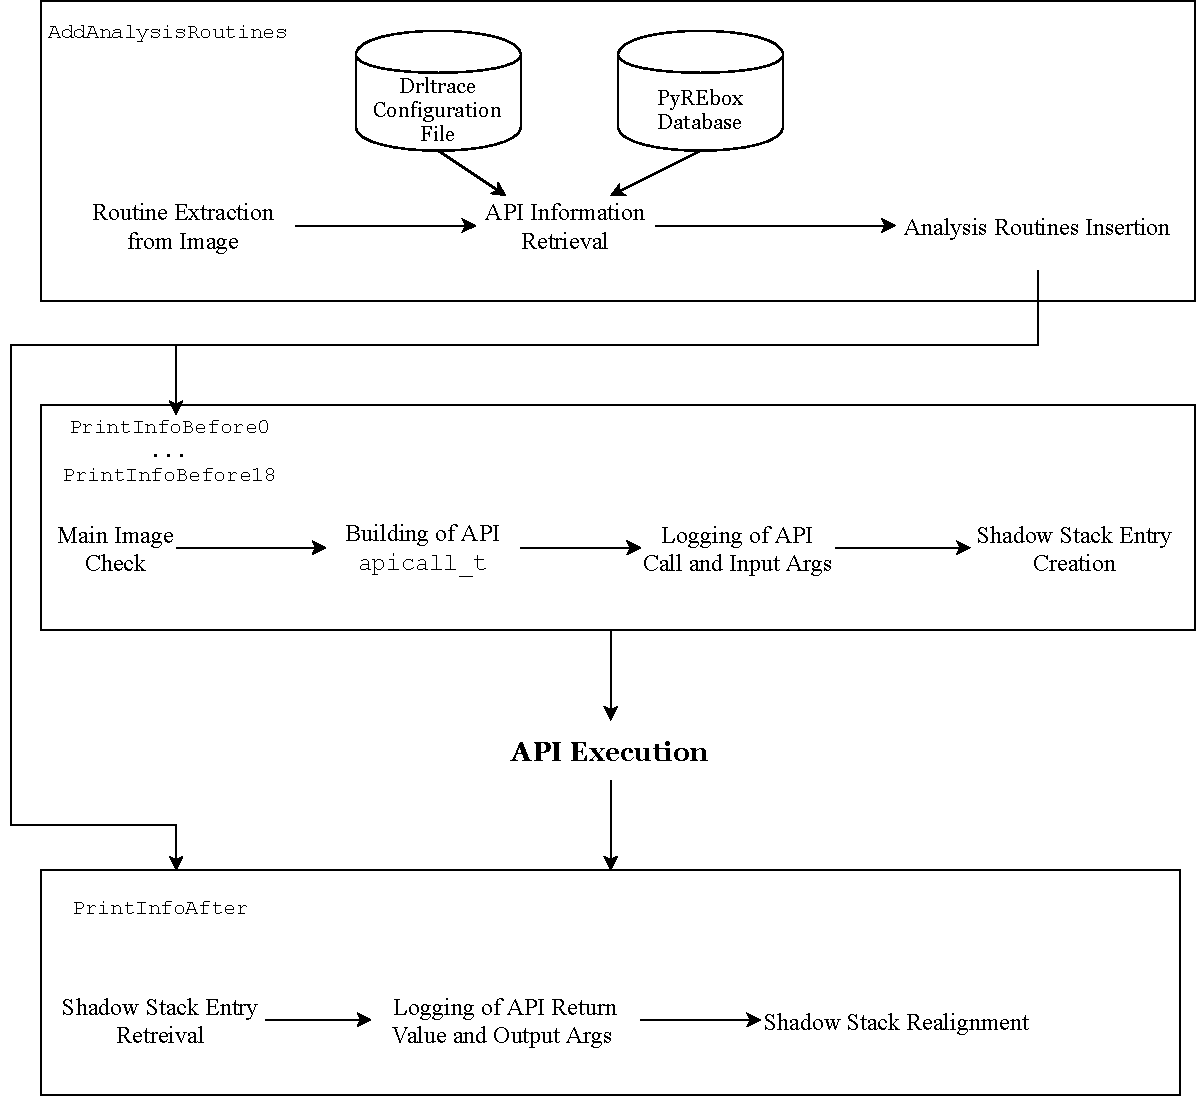
\includegraphics[scale=0.662]{Figures/APITracing.pdf}
\caption{\textit{APIs Tracing Workflow}}
\end{figure}

 
When tracing APIs, most of the concepts seen in Native API tracing also apply, but there are also significant differences, both in the steps that were carried out and in the Pin APIs which were employed, as it can be observed from the diagram in \textit{Figure 3.4}.

Now let us illustrate the actions being performed during API tracing by analyzing in detail each one of the three main blocks of \textit{Figure 3.4}.

\subsection{APIs Instrumentation}

The first step taken towards APIs tracing is APIs instrumentation, i.e. placing analysis routines before and after the APIs' execution. To do this, a specific function was embedded in Blue Pill's image callback (the notion of image callback was previously introduced in Section 3.3.1). Such function, named \texttt{AddAnalysisRoutines}, performs the following actions for every DLL being loaded:

\begin{enumerate} 
\item It inspects the symbol table, i.e. the DLL's exports. To this end, Pin symbol objects (\texttt{SYM}s) are employed, which provide information about function symbols in the applications \cite{Pin}.
\item For every symbol object, it retrieves the corresponding routine (\texttt{RTN}) object. In fact, in Pin a \texttt{RTN} represents a function usually generated by a compiler for a procedural programming language, e.g C \cite{Pin}. To retrieve the aforementioned \texttt{RTN} object, the \texttt{RTN\_FindByAddress} API was utilized, which takes as input a \texttt{RTN} memory address and returns an handle to the found \texttt{RTN}. Such memory address was determined by adding the symbol's RVA (obtained via \texttt{SYM\_Value}) to the lowest image address (fetched through \texttt{IMG\_LowAddress}).  
\item For every routine object, it retrieves the corresponding name via \texttt{RTN\_name} and checks whether or not the API being represented is "known", i.e. a source of information associated to the API exists.

\begin{itemize}
\item If the API is not "known", it adds an analysis routine just before the API's execution, which simply logs the value of a user-specified number of args (four by default), exactly like what happens in NTAPIs tracing.
\item If the API is "known", it adds analysis routines before and after the API's execution, which log detailed information relative to the API, including the arguments' input and output values. 
\end{itemize}
 
\end{enumerate}

Having given a general outline on how \texttt{AddAnalysisRoutine} works, let us now describe its underlying details.

Similarly to what occurs for NTAPI tracing, in order to log as much information as possible and to correctly record the arguments' values, it is necessary to have a source of API information, providing some kind of assistance during the tracing activity. When dealing with APIs, BlueTracer allows the user to choose between two possible sources of API information: \textit{drltrace}'s configuration file or the data extracted from \textit{PyREbox}'s database. By default, the latter is employed as it embodies a greater amount of information, including variable names and named constants' enumerations.

\textit{drltrace} (already mentioned in section 2.3) comes with its own external configuration file, in which each line contains information relative to an API, as it can be observed from the sample configuration file entry below (\textit{Listing 3.9}).      
\\
\lstset{
    language=C++,
    frame=single, % draw a frame at the top and bottom of the code block
    tabsize=4, % tab space width
    showstringspaces=false, % don't mark spaces in strings
    numbers=none, % display line numbers on the left
    commentstyle=\color{ao}, % comment color
    keywordstyle=\color{blue}, % keyword color
    stringstyle=\color{red}, % string color
    basicstyle=\footnotesize\ttfamily,
    basewidth = {.48em}
}
\begin{lstlisting}[caption={Sample entry in \textit{drltrace} configuration file},captionpos=b]
bool|GetUILanguageInfo|DWORD|wchar*|__out wchar*|__inout DWORD*|__out DWORD*
\end{lstlisting}
\lstset{
    language=C++,
    frame=tb, % draw a frame at the top and bottom of the code block
    tabsize=4, % tab space width
    showstringspaces=false, % don't mark spaces in strings
    numbers=left, % display line numbers on the left
    commentstyle=\color{ao}, % comment color
    keywordstyle=\color{blue}, % keyword color
    stringstyle=\color{red}, % string color
    basicstyle=\footnotesize\ttfamily,
    basewidth = {.48em}
}

Each piece of information in an entry is separated by \texttt{|}. The first bit of data is the API's return type, the second is the API's name and the rest of the entry is made up by the arguments' types. In particular, the \texttt{\_\_out} token is used to mark output arguments, while \texttt{\_\_inout} is utilized to identify input and output arguments. In case there is no token, it means that the argument is just an input one. 

Before API instrumentation takes place, BlueTracer parses the aforementioned configuration file and, for every entry, builds a \texttt{sysinfo\_arg\_t struct} (\textit{Listing 3.2}) for each argument in the entry. It was decided to reuse \texttt{sysinfo\_arg\_t struct} since its fields were fitting with respect to the arguments' information which had to be stored. Therefore, after this parsing process, each configuration file entry is represented by an <API name, \texttt{vector} of \texttt{sysinfo\_arg\_t}s> pair. Such pairs are then utilized to build an hash map, which maps the API name to the corresponding arguments. This hash map is used in step 3 of the APIs instrumentation process to, given the API name, fetch the appropriate information. In particular, it is important to note that, from a performance point of view, it is much better to include the information retrieval operations in the image instrumentation function, rather than in the analysis ones, as the former are executed just once for every image, while the latter are invoked each time an API is called by the pinned application.

The other source of API information employed by BlueTracer is \textit{PyREbox}'s database. \textit{PyREbox} is a Python scriptable reverse engineering sandbox based on QEMU and VMI techniques, the goal of which is to provide support for reverse engineering through its dynamic analysis capabilities \cite{Pyrebox}. \textit{PyREbox} is equipped with its own API tracer, which relies on the information contained in a sqlite database to correctly log the APIs' parameters. Such database was, in turn, generated by utilizing as its core the data from the \textit{Deviare}\footnote{Deviare is an open-source hooking engine for instrumenting arbitrary \texttt{Win32} functions \cite{Deviare}} project and then employing a crawler for parsing the Microsoft online documentation with the goal of marking which parameters are input parameters and which are output parameters. The resulting database is incredibly richer in API information than \textit{drltrace}'s configuration file. In fact, the number of APIs for which data is stored is much higher, argument names are also included, as well as the contents of named constants' enumerations, information which \textit{drltrace}'s configuration file does not provide at all.

In order to extract information relative to the APIs from PyREbox's database, a Python script was employed, which, for every API, instantiates a \texttt{libcall\_info\_t struct} (\textit{Listing 3.10}) in a \texttt{.cpp} file.
\\
\begin{lstlisting}[caption={\texttt{struct} containing API-related information from PyREbox's database},captionpos=b]
typedef struct _libcall_info_t {
	const char* func_name;     			// API name
	int argnum;				   			// Number of Args
	libcall_arg_info_t lib_args[19];	// Array of arguments
} libcall_info_t
\end{lstlisting}
\vspace{1cm}

The most important field of such \texttt{struct} is surely the arguments' array, which is made up of \texttt{libcall\_arg\_info\_t} data structures (\textit{Listing 3.11}) containing the information relative each argument of an API, including an entry specific for the return value data. The array size was set to 19, since it was observed from the database data that the API with the most parameters had 18 arguments. This time, it was decided not to reuse NTAPI's \texttt{sysinfo\_arg\_t struct} (\textit{Listing 3.2}) to store the API's arguments information due to its lack of the field storing the argument name. 
\\
\begin{lstlisting}[caption={\texttt{struct} containing information associated to an API argument},captionpos=b]
typedef struct _libcall_arg_info_t {

	int arg_num;				// Arg Ordinal
	const char* arg_name;		// Arg Name
	int arg_type;             	// Arg Type
	char* arg_type_name;		// Arg Type Name
	int size;					// Size
	bool in_out_flag;			// Input/Output Flag

} libcall_arg_info_t;
\end{lstlisting}   

Although \texttt{libcall\_arg\_info\_t}'s fields seem to be pretty self-explanatory, let us quickly go through them to reveal some details which are not so obvious:

\begin{itemize}
\item \texttt{arg\_num} is an \texttt{int} which contains the argument's ordinal. In case the return value is being represented, it is set to -1.
\item \texttt{arg\_name} is a string containing the argument name as reported by Microsoft's official documentation.
\item \texttt{arg\_type} is an \texttt{int} from an enumeration representing the argument's type. In particular, differently from the strategy adopted from Native APIs, in case of a pointer the \texttt{NKT\_DBOBJCLASS\_Pointer} enumeration member is ORed with an \texttt{int} representing the pointed type. The same thing happens in case of a pointer to a pointer but with the \texttt{NKT\_DBOBJCLASS\_PointerPointer} flag being used instead. This was done to reflect how API information is stored inside the database.
\item \texttt{arg\_type\_name} is a string which is used in the three specific scenarios below, according the type of the argument, and is \texttt{null} otherwise:
\begin{enumerate}
\item To store the symbolic name of an enumeration.
\item To store the \texttt{struct} type name.
\item To store the \texttt{union} type name.
\end{enumerate}
\item \texttt{size} is an \texttt{int} storing the argument's size. In case of a pointer (or a pointer to a pointer) the size of the pointed type is stored.
\item \texttt{in\_out\_flag} is a \texttt{bool} which is set to \texttt{INOUT} (i.e \texttt{true}) if the represented argument is an output argument and \texttt{IN} (i.e. \texttt{false}) otherwise. This means that, by default, all the arguments are considered as input arguments and are therefore traced before the API execution, while only the arguments for which \texttt{in\_out\_flag} is \texttt{true} are traced after the API's execution.
\end{itemize}

To give a better idea on how API data is represented, an instance of \texttt{libcall\_arg\_info\_t} containing the information associated to \texttt{WriteFileEx} can be observed below (\textit{Listing 3.12}).
\\
\begin{lstlisting}[caption={Instance of \texttt{libcall\_arg\_info\_t} relative to \texttt{WriteFileEx}},captionpos=b]
	{ "WriteFileEx",5,
	{ 
		{-1, "Return value", NKT_DBFUNDTYPE_SignedDoubleWord, 0, 4, INOUT },
		{0, "hFile", NKT_DBFUNDTYPE_UnsignedDoubleWord, 0, 4, IN },
		{1, "lpBuffer", NKT_DBFUNDTYPE_Void | NKT_DBOBJCLASS_Pointer, 0, 0, IN },
		{2, "nNumberOfBytesToWrite", NKT_DBFUNDTYPE_UnsignedDoubleWord, 0, 4, IN },
		{3, "lpOverlapped", NKT_DBOBJCLASS_Struct | NKT_DBOBJCLASS_Pointer,
		 "_OVERLAPPED", 160, INOUT },
		{4, "lpCompletionRoutine", NKT_DBOBJCLASS_Typedef, 0, 0, IN },
	}
	}
\end{lstlisting}

Due to the high amount of APIs for which information was stored in the \texttt{PyREbox} database, it was decided to group API data by DLL. Specifically, for every DLL a corresponding \texttt{.cpp} file was created to store the API-related information under the form of \texttt{libcall\_arg\_info\_t} instances, one for each "known" API exported by that DLL. Furthermore, in order to make API data retrieval more efficient, it was chosen to employ a two-level hash map approach for this purpose. Given the DLL name (easily obtainable in the image callback via the use of \texttt{IMG\_Name}), the first level hash map is utilized to retrieve the DLL-specific second level hash map, which, in turn, maps the API name to the appropriate \texttt{struct} instance (\textit{Figure 3.5}). This is how API information retrieval is carried out in case \textit{PyREbox} database is used as API data source.
\\
\begin{figure}[h]
\centering
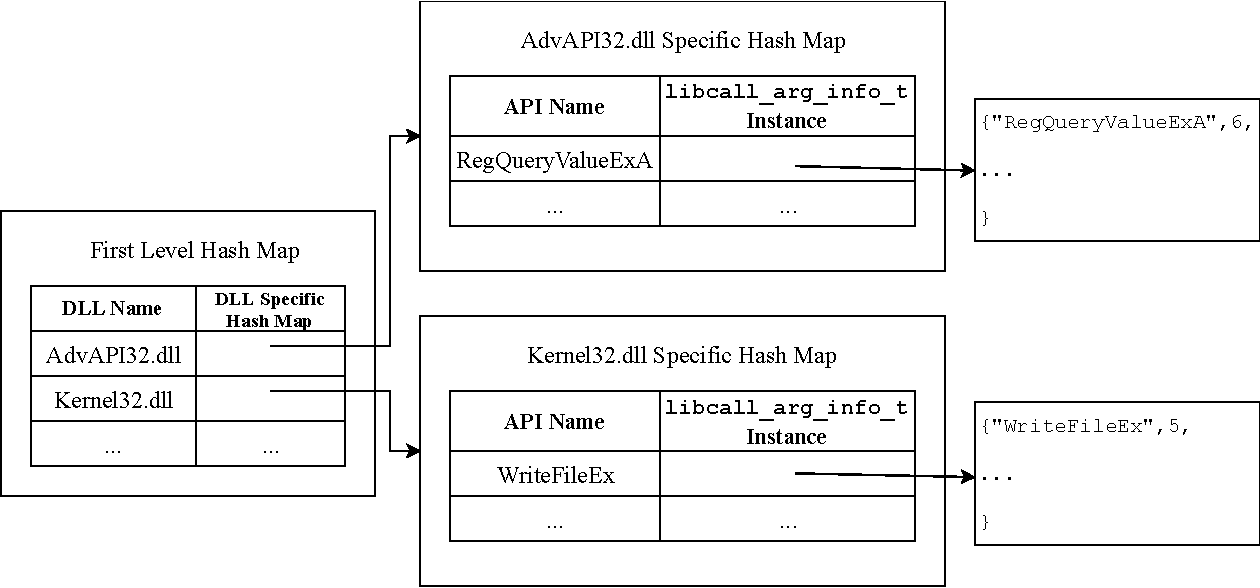
\includegraphics[width=1\textwidth]{Figures/HashMap.pdf}
\caption{\textit{PyREbox API Information Retrieval}}
\end{figure}

Let us conclude this section by explaining how analysis routines are inserted before and after the API execution during the API instrumentation procedure outlined in page 31. In BlueTracer such operation heavily relies on the use of the \texttt{RTN\_InsertCall}, which allows to insert analysis functions relative to a \texttt{RTN} object. This API takes as input the following parameters:
\begin{itemize}
\item The routine object (\texttt{RTN}) representing the function under analysis.
\item A member of the \texttt{IPOINT} enumeration which determines where the analysis function is inserted in relation to the instrumented object. It can be either \texttt{IPOINT\_BEFORE}, in which case the analysis code is placed before the instrumented function, or \texttt{IPOINT\_AFTER}, in which case the analysis code is placed after the instrumented function.
\item The analysis function to be called.
\item The arguments to pass to the analysis function, specified via members of the \texttt{IARG\_TYPE} enumeration. If the analysis function is placed before the instrumented object, then such arguments may also include the parameters' values of the function being instrumented. However, for this to occur the pair <\texttt{IARG\_FUNCARG\_ENTRYPOINT\_VALUE}, argument number> needs to be included for each of the analyzed function's parameters. Conversely, to obtain the instrumented function's result, \texttt{IARG\_FUNCRET\_EXITPOINT\_VALUE} is required. Obviously, this is possible only if the analysis function is placed after the instrumented object.
\end{itemize}

In BlueTracer, the number of arguments of the API being traced is known only after the API-related information has been retrieved. Because of this and given Pin's way of passing the arguments to the analysis functions, a \texttt{switch} had to be employed when adding analysis functions before the API execution. Such \texttt{switch}, given the API arguments' number, places the appropriate analysis function, i.e. the one with the number of <\texttt{IARG\_FUNCARG\_ENTRYPOINT\_VALUE}, argument number> pairs equal to the number of arguments the API takes. This is done in order to ensure that the analysis function receives all the values of the API's arguments before the API's execution. As a result, in BlueTracer there are 19 (one for zero arguments as well) different API \texttt{IPOINT\_BEFORE} analysis functions, named \texttt{PrintInfoBefore[Arguments' Number]}, which vary only in the number of APIs' argument values they receive in input. Obviously this is true just for "known" APIs. In case the API under analysis is not "known", then the number of API argument values is always the same and the \texttt{switch} is not required.

Let us now dissect an invocation of \texttt{RTN\_InsertCall} to further clarify how BlueTracer adds analysis code before the execution of an API (\textit{Listing 3.13}).  
\begin{lstlisting}[caption={\texttt{RTN\_InsertCall} invocation to add analysis code before an API's execution},captionpos=b]
RTN_InsertCall(rtn, IPOINT_BEFORE, (AFUNPTR)PrintInfoBefore[Number of API Args],
 	IARG_FAST_ANALYSIS_CALL,
	IARG_ADDRINT, argNumber,
	IARG_ADDRINT, libPointer, IARG_ADDRINT, rtn_name, IARG_ADDRINT, img_name,
	IARG_REG_VALUE, REG_STACK_PTR,
	IARG_THREAD_ID,
	IARG_RETURN_IP,
	[Number of API Args]_ARGS
	IARG_END);
\end{lstlisting}

In particular, the arguments which are passed to the analysis routine are:
\begin{itemize}
\item \texttt{IARG\_FAST\_ANALYSIS\_CALL}. This is not a real argument but rather a way to enable faster linkage for calls to analysis functions with the objective of improving performance \cite{Pin}.
\item \texttt{argNumber}, a constant value containing the number of the analyzed API's arguments.
\item \texttt{libPointer}, a reference to the previously retrieved data structure containing API-related data.
\item \texttt{rtn\_name}, the API name.
\item \texttt{img\_name}, the DLL name.
\item The stack pointer value before the API's execution, given by the \texttt{<IARG\_REG\_VALUE, REG\_STACK\_PTR>} pair. This is necessary for the shadow stack management, which will be detailed in the next section.
\item The thread ID assigned by Pin for the calling thread, passed via \texttt{IARG\_THREAD\_ID}. This is necessary in order to access the thread local storage from the analysis function.
\item The API return address, provided by \texttt{IARG\_RETURN\_IP}. This is employed in the main image check, similarly to what explained in Section 3.3.1.
\item The API argument values. In order to make the code more readable a macro was used in this case.
\end{itemize}

For what concerns the addition of analysis code after the API's execution, the aforementioned \texttt{switch} is not necessary since \texttt{IARG\_FUNCRET\_EXITPOINT\_VALUE} is valid only at the entry point of an analysis routine and, therefore, no API argument value is passed at this stage. The analysis function which is placed after the API's execution, named \texttt{PrintInfoAfter} essentially receives the same parameters as the ones from \textit{Listing 3.13}, with the major difference that the API's return value is passed via \texttt{IARG\_FUNCARG\_EXITPOINT\_VALUE} instead of the API arguments' values.

\subsection{API Analysis before Execution}

In this section we will describe how APIs are analyzed before execution, i.e. the main steps that are carried out in the \texttt{PrintInfoBefore} functions, an overview of which is given in \textit{Figure 3.4}.
The workflow in this case is mostly the same as the one for NTAPIs' analysis, with one major difference, that is the introduction of a shadow stack used to store API entries in the thread local storage, which will be motivated later in the section.

The first thing which is done is determining whether or not the API under analysis has been invoked directly from the main executable of the Pin application. The concepts involved here are exactly the same as the ones applying to the main image check done for Native APIs, which was detailed in \textit{Section 3.3.1}. In short, it is checked if the API's return address, which is passed to the analysis function through the use of \texttt{IARG\_RETURN\_IP}, falls into the main executable memory address range, which was previously determined via \texttt{IMG\_HighAddress} and \texttt{IMG\_LowAddress}.

Afterwards, similarly to what occurs when logging "known" Native APIs, a \texttt{apicall\_t struct} (\textit{Listing 3.14}) representing the specific API being traced is allocated and initialized. The fields of such \texttt{struct} are all trivial and, as what done for Native API tracing, the API arguments are represented via a \texttt{drsys\_arg\_t} (\textit{Listing 3.6}) array with size \texttt{MAX\_ARGS\_CONFIG} (i.e. 18) as this is the maximum number of observed arguments for any "known" API. In particular, the \texttt{drsys\_arg\_t struct} could be reused in the context of APIs since, unlike \texttt{sysinfo\_arg\_t}, its fields could hold all API arguments' data, both from the \textit{drltrace} configuration file and the \textit{PyREBox} database, including the argument name. 
\\
\begin{lstlisting}[caption={\texttt{struct} representing the API being traced},captionpos=b]
typedef struct _apicall_t {;

	const char* img_name;							// DLL Name
	const char* rtn_name;							// API Name

	drsys_arg_t arguments[MAX_ARGS_CONFIG];			// Array of Arguments
	drsys_arg_t retval;								// Return Value
	int count;										// Arg Count

} apicall_t;
\end{lstlisting}

Such \texttt{struct} is initialized utilizing the API-related information, which was fetched beforehand during instrumentation and was passed to the analysis function via \texttt{libPointer}, as well as the values of the API arguments, which were provided to the analysis function through \texttt{IARG\_FUNCARG\_ENTRYPOINT\_VALUE} as already discussed in \textit{Section 3.4.1}.

Then, the logging of the API proceeds exactly the same as for Native APIs: the API call is recorded employing an identical log format in order to maintain uniformity and the input values of the arguments are logged through the use of a \texttt{print\_arg} function operating exactly in the same way as the one in \textit{Listing 3.7}.

As previously hinted at, the major element which distinguishes API tracing from Native API tracing is that the former employs a shadow stack to store in the thread local storage references to the data structures representing the APIs being traced. Let us explain in detail the motivation behind such choice. It is typical for an API to call another API during its execution, forming a sort of nesting. For this reason, just storing in the thread locale storage the reference relative to the next API to be executed is not enough as this would lead to the analysis of just the most "inner" API, completely ignoring the "outer" APIs which invoked the "inner" one. Therefore, it is necessary to store not just the reference corresponding to the next API in line to be executed but rather all the references relative to the APIs for which execution has started and not yet finished. A fitting data structure to solve this issue is a shadow stack, where, for each API, the corresponding data structure is placed on top of the stack before its execution and popped from the stack after its execution has terminated, allowing both "inner" and "outer" APIs to be traced. This is why each thread has access to its own shadow stack via the \texttt{shadowStack} field in the thread local data (\textit{Listing 3.1}).

Therefore, in light of what just stated, the last operations which are done when tracing an API before its execution are allocating a shadow stack entry (\textit{Listing 3.15}), initializing it and placing it on top of the shadow stack in the thread local data, so that it can be retrieved after the API's execution.
\\
\begin{lstlisting}[caption={\texttt{struct} representing a shadow stack entry},captionpos=b]
typedef struct _stackEntry {
	apicall_t* apiInfo;    // API Call Reference
	ADDRINT  currentSP;    // Stack Pointer Register Content
	THREADID threadID;     // Thread ID
	uint api_counter;	   // Call Counter
} stackEntry;
\end{lstlisting}       

\texttt{stackEntry}'s fields are all, once again, self-explanatory. A big role in the stack realignment procedure is placed by the \texttt{currentSP} field, as it will be explained in the next section. Such field stores the stack pointer's value before the API's execution, which was passed to the analysis function with the <\texttt{IARG\_REG\_VALUE}, \texttt{REG\_STACK\_PTR}> pair.

\subsection{API Analysis after Execution}



\iffalse
- Shadow Stack Realignment
-> Remove all entries BEFORE in the stack
-> Remove all entries with a lower stack pointer
\fi

The resulting log format is very similar to the one employed for Native APIs in order to mantain the format uniform throughtout the log.

\section{Callback and APC} 

In this section callbacks and APCs -> Both rely on the use of the OnContextChange API.

\subsection{Callbacks}
\subsection{APC}

\iffalse
\section{Tool Configuration}
\fi
